\documentclass{article} % \documentclass{} is the first command in any LaTeX code.  It is used to define what kind of document you are creating such as an article or a book, and begins the document preamble

\usepackage{amsmath} % \usepackage is a command that allows you to add functionality to your LaTeX code
\usepackage{enumitem}
\usepackage{graphicx}

\title{Relazione progetto programmazione per il web 2021/2022} % Sets article title
\author{
  D'Ales Alessio\\
  \texttt{1903817}
  \and
  Albertini Tommaso\\
  \texttt{1893643}
  \and
  Iltchev Federico\\
  \texttt{1842707}
}
\date{} % Sets date for date compiled 

\renewcommand{\labelenumii}{\theenumii}
\renewcommand{\theenumii}{\theenumi.\arabic{enumii}.}


% The preamble ends with the command \begin{document}
\begin{document} % All begin commands must be paired with an end command somewhere
    \maketitle % creates title using information in preamble (title, author, date)
    

    \section{Introduzione}

    OutOfMemory è un sito web in cui si possono fare domande riguardo a vasti argomenti di programmazione.
    Il sito fornisce la possibilità agli utenti di chiedere o rispondere a domande e di lasciare un like ai post oppure alle risposte
    più utili. Gli utenti hanno un profilo in cui possono visualizzare i like ricevuti e i post pubblicati.

    \section{Il diagramma ER}


    \begin{figure}[h!]
        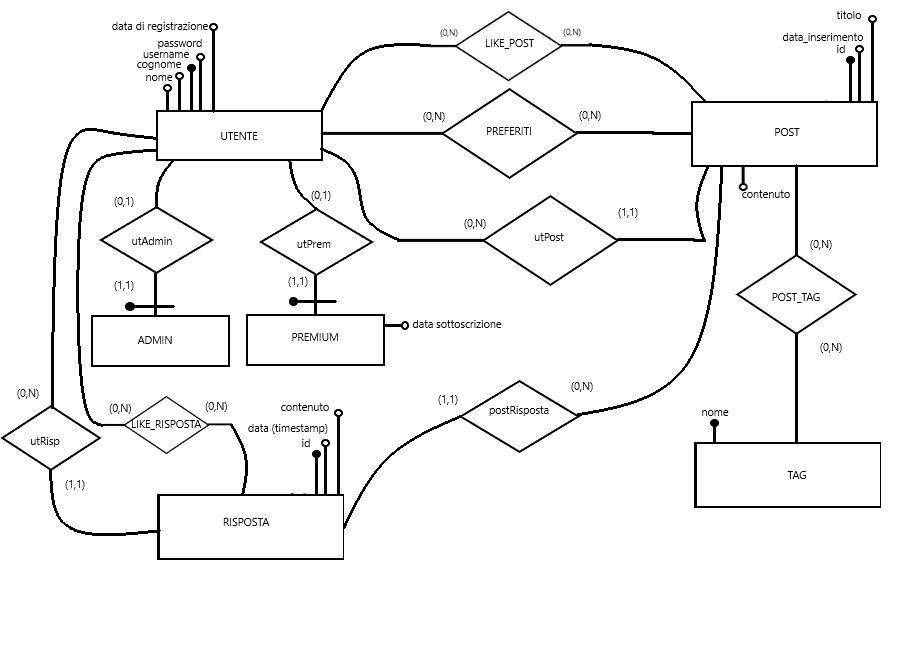
\includegraphics[width=\linewidth]{PWEB-ER.png}
    \end{figure}

    Il database si compone delle seguenti tabelle:

    \begin{enumerate}[label*={\arabic*.}]
        \item \textbf{UTENTE}
            \begin{enumerate}[label*={\arabic*.}]
                \item nome: mantenimento di informazioni base dell'utente (facoltativo)
                \item cognome: mantenimento di informazioni base dell'utente (facoltativo)
                \item username: chiave primaria , usato come riconoscimento utente univoco
                \item data di registrazione
                \item password: viene salvato l'hash della password ottenuto con BCrypt
            \end{enumerate}
        \item \textbf{ADMIN}
            \begin{enumerate}[label*={\arabic*.}]
                \item username: FK per inserire un utente nella categoria "admin" 
            \end{enumerate}
        \item \textbf{PREMIUM}
            \begin{enumerate}[label*={\arabic*.}]
                \item data di sottoscrizione: viene salvata la data in cui l'utente diventa premium, per un possibile scenario in cui si può pagare per diventarlo
                \item username: FK per inserire un utente nella categoria "premium" 
            \end{enumerate}
        \item \textbf{POST}
            \begin{enumerate}[label*={\arabic*.}]
                \item id: (serial) auto incrementale come chiave primaria per riconoscimento post univoco
                \item premium: (booleano) se un post è rivolto ad utenti premium
                \item creatore: FK per inserire l'username del creatore del post
                \item data: (timestamp) che verrà usato per ordinare i post in base alla data
                \item titolo
                \item contenuto
            \end{enumerate}    
        \item \textbf{PREFERITI}
            \begin{enumerate}[label*={\arabic*.}]
                \item utente: FK per indicare un utente esistente  
                \item id post: FK per indicare un post esistente 
            \end{enumerate}
        \item \textbf{POSTTAG}
            \begin{enumerate}[label*={\arabic*.}]
                \item tag: FK per indicare un tag esistente  
                \item id post: FK per indicare un post esistente 
            \end{enumerate}
        \item \textbf{RISPOSTA}
            \begin{enumerate}[label*={\arabic*.}]
                \item id: (serial) auto incrementale come chiave primaria per riconoscimento risposta univoca
                \item creatore: FK per inserire l'username del creatore della risposta
                \item data: (timestamp) che verrà usato per ordinare le risposte in base alla data
                \item contenuto
            \end{enumerate}
        \item \textbf{TAG}
            \begin{enumerate}[label*={\arabic*.}]
                \item nome: per l'inserimento successivo di tag personalizzati
            \end{enumerate}
        \item \textbf{LIKEPOST}
            \begin{enumerate}[label*={\arabic*.}]
                \item username
                \item id post
            \end{enumerate}
        \item \textbf{LIKERISPOSTA}
            \begin{enumerate}[label*={\arabic*.}]
                \item username
                \item id risposta
            \end{enumerate}
    \end{enumerate}


    \section{Funzionalità}

    \subsection{Il database}
    Il database si occupa di salvare tutte le informazioni che necessitano persistenza, come i dati degli utenti,
    dei post e delle risposte. \\

    \textbf{Tecnologia utilizzata:} MYSQL \\
    \textbf{Risponde al requisito:} Database degli utenti con diversi diritti di accesso, mantenimento di informazioni relative a un utente,
    Database di risorse caricabili dall’admin e accessibili agli user, eventualmente con diversi vincoli

    \subsection{Navigation bar e footer}
    Navigation bar e footer sono due pagine jsp incluse e persistenti in ogni pagina tramite azione standard include.
    Permettono la navigazione in tutto il sito e funzioni come la ricerca, il passaggio alla lingua inglese e il login. \\

    \textbf{Tecnologia utilizzata:} JSP, azioni standard \\
    \textbf{Risponde al requisito:} Presenza di pagine informative raggiungibili da ogni altra pagina

    \subsection{Login}
    La pagina di login permette l'inserimento di username e password con successivo riconoscimento
    dell'utente in caso di password corretta. Il meccanismo prevede il recupero dell'hash salvato nel database
    associato al nome utente che viene confrontato con la password appena inserita tradotta in hash dall'algoritmo
    di hashing. Questa risorsa viene bloccata da un filtro nel caso in cui l'utente sia già entrato con le sue credenziali. \\

    Un utente può essere riconosciuto come utente premium, come utente admin o come utente base.
    Un utente base visualizza solo i post base cioè inseriti da utenti base.
    Un utente premium può inserire post premium e può visualizzare tutti i post.
    Un utente admin può visualizzare tutto, inserire post premium e cancellare qualsiasi cosa (post e risposte)
    

    \textbf{Tecnologia utilizzata:} Servlet, Filtri, JDBC, JSP, sessioni \\
    \textbf{Risponde al requisito:} Database degli utenti con diversi diritti di accesso, Mantenimento di informazioni relative a un utente
    
    \subsection{Registrazione}
    La registrazione dell'utente prevede l'inserimento di due campi facoltativi (nome e cognome) e tre campi obbligatori,
    quali username e la coppia di password che deve combaciare. Se l'username scelto non esiste già, allora inserisce
    nel database tutti i dati immessi nel form; altrimenti restituisce una pagina di errore. \\
    
    \textbf{Tecnologia utilizzata:} Servlet, Filtri, JDBC, sessioni \\
    \textbf{Risponde al requisito:} Database degli utenti con diversi diritti di accesso, Mantenimento di informazioni relative a un utente

    \subsection{Traduzione}

    E' possibile visualizzare i testi statici in lingua italiana e inglese; la lingua corrente è memorizzata in un attributo
    di sessione. Cliccando sulla bandiera corrispondente nel footer viene impostato l'attributo di sessione e tutte le pagine
    useranno i testi tradotti in inglese. \\

    \textbf{Tecnologia utilizzata:} JSP, sessioni, JSP taglib fmt e c, file properties (contiene i testi nelle varie lingue) \\
    \textbf{Risponde al requisito:} Gestione della localizzazione


    \subsection{Bacheca post}

    La bacheca post visualizza tutti i post inseriti dagli utenti, divisi in tre categorie: \\
    post risposti : hanno ricevuto almeno una risposta \\
    post non risposti : non hanno ricevuto nessuna risposta \\
    post premium : bloccati dall'accesso e dalla visualizzazione agli utenti base; questi post protetti possono servire in uno scenario tipo in cui un utente definito "esperto" vuole che a sua volta rispondano solo utenti "esperti" \\
    Vengono visualizzati i tag associati al post e l'utente che lo ha creato 
    
    Ogni pagina genera al massimo 5 post, è possibile lo scorrimento delle pagine.
    Ogni post è un hyperlink al dettaglio post contenente la domanda e le relative risposte.

    E' divisa in tre tab: \\
    Tutti : visualizza tutti i post \\
    Preferiti : visualizza solo i post contrassegnati come preferiti, uno scenario tipico è l'utente che vuole salvare uno specifico post per una successiva visualizzazione \\
    Tag : Visualizza il risultato di una ricerca per titolo o per tag \\
    
    


    \textbf{Tecnologia utilizzata:} JSP (visualizzazione dati), JDBC (recupero dati post), URL rewriting \\
    \textbf{Risponde al requisito:} Database di risorse caricabili dall’admin e accessibili agli user, eventualmente con diversi vincoli, Categorizzazione delle risorse, user-generated content, con limitazioni su chi può inserire contenuti, Mantenimento di carrello e preferenze persistente

    \subsection{Inserimento post}
    Gli utenti possono scrivere post attraverso la compilazione di un form. \\
    Il form da compilare è composto da 4 campi: \\
    Titolo: il titolo del post\\
    Contenuto: la domanda scritta dall'utente \\
    Tags: il linguaggio utilizzato per il codice \\
    Premium: visualizzato solo da utenti premium, permette di scegliere la visibilità della domanda \\
    \textbf{Tecnologia utilizzata:} Servlet (inserimento nel DB), JDBC \\
    \textbf{Risponde al requisito:} 
    user-generated content, con limitazioni su chi può inserire contenuti

    \subsection{Rispondere ai post}
    Gli utenti che hanno effettuato il login possono rispondere a un post, tramite metodo post.
    Gli utenti premium sono gli unici che possono rispondere a tutti. \\

    \textbf{Tecnologia utilizzata:} Servlet (inserimento risposta nel DB), JDBC \\
    \textbf{Risponde al requisito:} user-generated content, con limitazioni su chi può inserire contenuti

    \subsection{Inserire un like ad un post o una risposta}
    Ogni post o risposta può ricevere un like dagli utenti, che si andranno a sommare
    al conto del creatore delle stesse. Questa funzionalità può servire in uno scenario tipo per far diventare
    un utente premium. Ad esempio raggiunti i 100 like, l'utente diventa "esperto" e ha una reputazione
    positiva. \\
    
    \textbf{Tecnologia utilizzata:} Servlet, JDBC , URL rewriting \\
    \textbf{Risponde al requisito:} Database degli utenti con diversi diritti di accesso

    \subsection{Aggiungere un post ai preferiti}
    Sui post vi è un campo "Aggiungi ai preferiti" in cui viene inserita una riga nella tabella preferiti.
    Viene anche controllato che non esista già. \\
    
    \textbf{Tecnologia utilizzata:} Servlet, JSP, JDBC \\
    \textbf{Risponde al requisito:} Mantenimento di preferenze persistenti \\

    \subsection{Rimuovere un post o una risposta}
    Una Servlet una volta premuto il tasto "Cancella Risposta" permette di rimuovere dal forum
    il post o la risposta ad un post. \\

    \textbf{Tecnologia utilizzata:} Servlet, JDBC \\
    \textbf{Risponde al requisito:} user-generated content, con limitazioni su chi può inserire contenuti

    \subsection{Scorrimento pagine nella bacheca}
    Gli utenti tramite il bottone, nell'URL viene salvato un attributo pagina in cui viene \\
    visualizzata solo quella pagina, e tramite URL rewriting, si viene reindirizzati alla pagine richiesta.\\
    
    \textbf{Tecnologia utilizzata:} JSP, URL Rewriting, JDBC \\
    \textbf{Risponde al requisito:} Presenza di pagine informative raggiungibili da ogni altra pagina 

    \subsection{Ricerca e Tag}

    La barra di ricerca è implementata nella navbar e permette la ricerca per titolo e per tag 
    I tag sono associati ad un post e inseriti durante la pubblicazione dello stesso. E' possibile filtrare per al più un tag e quindi visualizzare tutti i post associati
    Ogni qual volta viene cercato qualcosa, viene salvato un cookie, per mostrare le ricerche recenti. \\

    \textbf{Tecnologia utilizzata:} JSP, JDBC, URL rewriting, cookies \\
    \textbf{Risponde al requisito:} Possibilità di navigazione tramite riferimenti fra le risorse, Presenza di pagine informative raggiungibili da ogni altra pagina, Possibilità di raccomandazioni su criteri diretti (tag), Possibilità di navigazione tramite riferimenti fra le risorse

    \subsection{Profilo}
    La pagina del profilo permette di visulizzare 
    nome: il nome e cognome facoltativi da inserire \\
    username: nome utente con cui si viene identificati nel forum\\
    post: numero post pubblicati\\
    likes: numero like ricevuti\\
    e da quanto fai parte della community \\
    \textbf{Tecnologia utilizzata:} JSP, JDBC \\
    \textbf{Risponde al requisito:} /
    
    \subsection{CSS}

    Per mantenere l'identità visiva del sito.

    \textbf{Tecnologia utilizzata:} CSS, bootstrap, fontawesome icons \\
    \textbf{Risponde al requisito:} Mantenimento di identità visiva dell’applicazione sulle varie pagine. 





\end{document} % This is the end of the document